\documentclass[utf8, seminar]{fer}
%\documentclass[utf8, zavrsni, upload]{fer}
\usepackage{booktabs}
\usepackage{indentfirst}
\usepackage{subcaption}
\usepackage{placeins}
\usepackage{float}
\usepackage{cite} % Za bibliografiju
\usepackage{url} % Za web adrese
\usepackage{listings}
\usepackage{caption}
\usepackage{tabularx}
\usepackage{amsmath}
\usepackage{amsfonts}
\usepackage{amssymb}
\usepackage{amsthm}
\usepackage{mathtools}
\usepackage{graphicx}
\usepackage{booktabs}
\usepackage{array}
\usepackage{longtable}
\usepackage{hyperref}
\usepackage{url}
\usepackage{fancyhdr}
\usepackage{setspace}
\usepackage{titlesec}
\usepackage{enumitem}
\usepackage{xcolor}
\setlocalecaption{croatian}{abstract}{Sažetak}

\usepackage{mathptmx} % Use Times New Roman font
\usepackage{setspace} % For setting line spacing
\singlespacing % Set line spacing to 1

% Smanjeni razmak između bullet-a
\setlist[itemize]{itemsep=0pt, parsep=0pt, topsep=0pt, partopsep=0pt}
\setlist[enumerate]{itemsep=0pt, parsep=0pt, topsep=0pt, partopsep=0pt}

\usepackage{titlesec} % To control the title spacing
\titlespacing*{\chapter}{0pt}{-30pt}{10pt}

\renewcommand{\figurename}{Slika}
\renewcommand{\bibname}{Literatura}
\renewcommand{\tablename}{Tablica}
\renewcommand{\contentsname}{Sadržaj}
\renewcommand\thepage{}

\title{Comparison of EDR tools}
\naslov{Usporedba alata za nadzor i intervenciju na krajnjim točkama (Endpoint Detection and Response)}
\brojrada{N/a}
\author{Ante Čavar}
\datum{lipanj, 2025.}
\mentor{prof.dr.sc. Stjepan Groš}

\begin{document}
\maketitle
% \zadatak{hr_0036540817_73.pdf}
\begin{zahvale}
Zahvaljujem se prijateljima i obitelji koji su mi bili podrška prilikom pisanja ovog rada.
\end{zahvale}
\newpage
\tableofcontents
\newpage
\mainmatter
\setcounter{page}{1}
\renewcommand\thepage{\arabic{page}}
% \chapter{Uvod}
\par Sigurnost web aplikacija je bitan dio razvoja moderne programske potpore. 
Kako se napadi na web aplikacije povećavaju iz dana u dan, potrebno je osim razumijevanja 
prijetnji i ranjivosti, imati i alate kojima ranjivosti a s njima i prijetnje možemo svesti na prihvatljivi minimum.

% \par Dva najraširenija takva alata trenutno dostupna javnosti su OWASP ZAP i Burp 
% Suite. OWASP ZAP (još znan i kao Zed Attack Proxy) je program otvorenog koda namijenjen
% za skeniranje web aplikacija tj.\ stranica. Produkt je organizacije \textit{Open Web Application 
% Security Project} (OWASP) te održavan kako od njih tako i od nemale skupine programera 
% i sigurnosnih stručnjaka iz cijelog svijeta. Alat pruža široki skup mogućnosti 
% za detekciju i testiranje ranjivosti u web aplikacijama. 

% \par Uz ZAP postoji Burp Suite, stariji i komercijalni alat namijenjen za sigurnosno testiranje 
% web aplikacija. Burp suite je razvila kompanija PortSwigger koja se također brine za njegovo 
% održavanje. Burp suite omogućuje pristup velikom rasponu alata, od skenera za traženje ranjivosti 
% pa sve do naprednih alata za \textit{fuzzing} i analizu web aplikacija. Najpoznatiji 
% alat među njima je \textit{proxy} koji omogućava korisnicima da presretnu HTTP/S zahtjeve 
% te izmijene HTTP/S zahtjeve i odgovore.

% \par OWASP ZAP i Burp Suite igraju važnu ulogu u području sigurnosti web aplikacija. 
% Prethodno navedeni i slični alati pomažu razvojnim inženjerima i sigurnosnim specijalistima u identifikaciji ranjivosti,
% razumijevanju površine napada (engl. \textit{attack surface}), vektora napada (engl. \textit{attack vector}) te u
% implementaciji efektivnih sigurnosnih rješenja.

% \par Cilj ovog rada je istražiti alat OWASP ZAP kao potencijalnu zamjenu za Burp Suite Professional testirajući
% mogućnosti oba alata u podjednakim uvjetima.
U ovom radu će se usporediti dva najraširenija alata za skeniranje i testiranje sigurnosti web aplikacija: OWASP ZAP i Burp Suite. 
Cilj je identificirati razlike u funkcionalnostima između ova dva alata, istražiti kako se mogu nadomjestiti funkcionalnosti koje ZAP 
nema, te opisati kako se pišu dodaci i proširuju mogućnosti ZAP-a. Na kraju, testirat će se nekoliko laboratorijskih vježbi koje se 
inače rješavaju pomoću alata Burp suite, koristeći ZAP.

Burp Suite je moćan, ali komercijalan alat koji zahtijeva skupu licencu za pristup svim funkcionalnostima. 
Za potrebe istraživanja i učenja, ovaj trošak može biti značajan. S druge strane, OWASP ZAP je alat otvorenog koda koji je besplatan 
za korištenje, ali potencijalno slabijih mogućnosti. Usporedbom ova dva alata, može se procijeniti koliko ZAP može biti održiva 
zamjena za Burp Suite u raznim scenarijima.

Najprije će se opisati osnovne funkcionalnosti oba alata. Zatim će se provesti nekoliko testova na različitim sigurnosnim scenarijima 
koristeći oba alata. Nakon toga, analizirat će se rezultati testova i usporediti performanse i mogućnosti ZAP-a i Burp Suite-a. 
Konačno, istražit će se mogućnosti proširenja funkcionalnosti ZAP-a kroz dodatke i skripte te predložiti rješenja za funkcionalnosti 
koje Burp Suite ima, a ZAP nema i pritom objasniti koji alat odabrati i zašto.
% \chapter{Funkcionalnosti}
Kako oba alata imaju pregršt funkcionalnosti navesti ću njihove najzanimljivije i najbolje implementirane funkcionalnosti 
koje će kasnije biti uspoređene.
\section{OWASP ZAP}
OWASP ZAP (još znan i kao Zed Attack Proxy) je program otvorenog koda namijenjen
za skeniranje web aplikacija tj.\ stranica. Produkt je organizacije \textit{Open Web Application 
Security Project} (OWASP) te održavan kako od njih tako i od nemale skupine programera 
i sigurnosnih stručnjaka iz cijelog svijeta. Alat pruža široki skup mogućnosti 
za detekciju i testiranje ranjivosti u web aplikacijama. Izgled ZAPa pri njegovom pokretanju vidljiv je na slici \ref{slk:owasp_start}.
\begin{figure}[H]
    \centering
    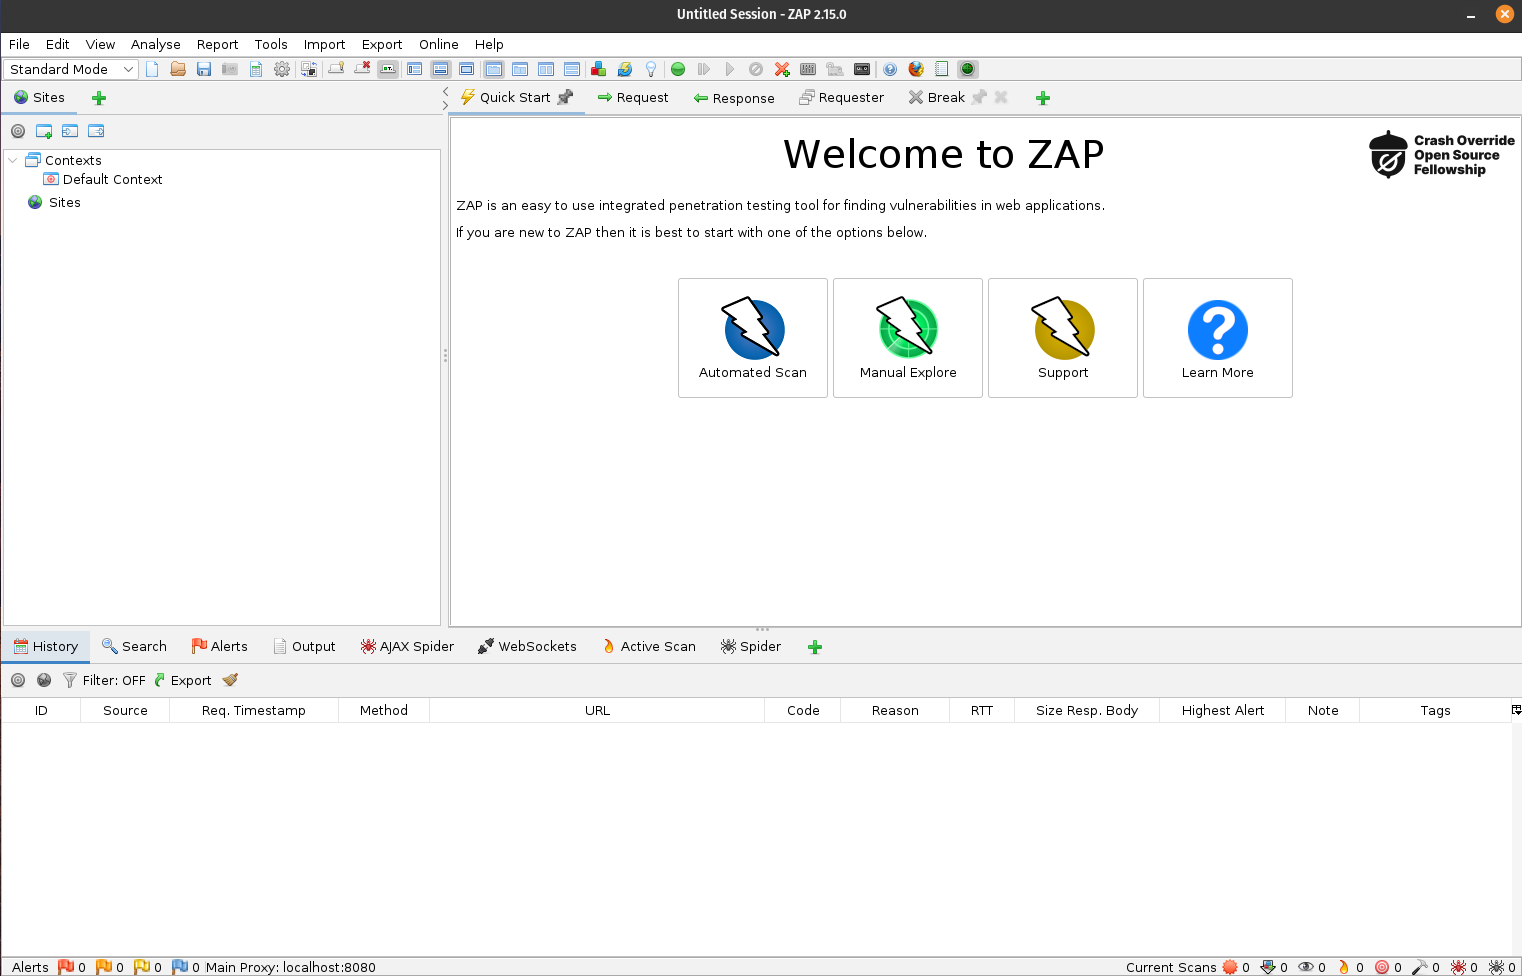
\includegraphics[width=0.8\textwidth]{slike/zap_start.png}
    \caption{Izgled OWASP ZAP-a pri pokretanju}
    \label{slk:owasp_start}
  \end{figure}

\subsection{Presretački \textit{proxy}}
\textit{Intercepting Proxy}, poznat i kao \textit{"Break"} u \textit{OWASP ZAP}-u, ključna je funkcionalnost koja omogućava 
korisnicima da presreću i pregledavaju \textit{HTTP/HTTPS} zahtjeve i odgovore između preglednika i web aplikacije. Ovo omogućuje 
korisnicima da detaljno pregledaju i modificiraju podatke prije nego što su oni poslani na server ili primljeni u pregledniku. 
Presretanje prometa korisno je za ručno testiranje sigurnosti jer omogućuje detaljnu analizu 
\textit{HTTP} zahtjeva i odgovora, uključujući zaglavlja, kolačiće, tijela zahtjeva i odgovore. 
Prije nego što se zahtjev pošalje ili odgovor primi, korisnici mogu ručno promijeniti podatke 
kako bi testirali različite scenarije.

Integrirani \textit{Heads-Up Display (HUD)} omogućava vizualno praćenje i kontrolu presretanja 
prometa direktno iz preglednika. Korisnici mogu simulirati razne vrste napada presretanjem i 
modificiranjem prometa, kao što su \textit{SQL} injekcije, \textit{XSS} napadi, \textit{CSRF}, i 
druge.\cite{ZAP_docs,zap_feat}


\subsection{Aktivno i pasivno skeniranje}% (engl. \textit{Active and Passive scan})}
Aktivno skeniranje (\textit{Active scan}) je ispitivanje ranjivosti pri kojem ZAP aktivno interaktira s aplikacijom ne bi li 
otkrila sve potencijalne sigurnosne prijetnje. Skeniranje uključuje slanje zahtjeva sistemu koji se testira (eng. \textit{system under test}, 
nadalje SUT) te analiziranje odgovora ne bi li dobili uvid u ranjivosti aplikacije.

Pasivno skeniranje (\textit{Passive scan}) je tip skeniranja gdje ZAP ne interaktira direktno s ijednim dijelom sustava na ijedan način.
Kako bi se pasivno prikupljale informacije, alat nadgleda mrežni promet za potencijalne ranjivosti. U pozadini alat i dalje nadgleda zahtjeve 
i odgovore no ne zamarajući korisnika s njima sve dok ne otkrije problem, onda podigne \textit{alert}.

Dobra stvar kod skeniranja u ZAP-u je mogućnost kontrole politike skeniranja. Ona nam omogućava da alatu pomognemo da bolje, lakše i brže pronađe ranjivosti koristeći 
znanje koje mi trenutno imamo, mogućnosti hardwera s kojim testiramo te vrste skenera koje imamo na raspolaganju. Te se politike mogu spremati te kasnije koristiti kao 
predložak u budućem testiranju.\cite{ZAP_docs,zap_feat}

\subsection{Skeniranje portova} % (engl. \textit{Port Scan})}
Funkcionalnost skeniranja portova u \textit{OWASP ZAP}-u obavlja skeniranje ranjivih portova nad \textit{SUT}-om kako bi utvrdio 
ranjive portove. U svojoj suštini radi isto što i određeni testovi za \textit{Nmap}\cite{nmap}, pronalazeći otvorene i zatvorene 
portove. Također, kao i \textit{Nmap}, može pronaći koji je trenutni servis na nekom od portova.

Služi kako bi se dobile dodatne informacije o potencijalnim vektorima napada. Pored toga, \textit{OWASP ZAP} može integrirati 
rezultate skeniranja portova sa svojim ostalim alatima za sigurnosno testiranje, omogućujući sveobuhvatnu analizu sigurnosti.

Za korištenje ove funkcionalnosti, potrebno je omogućiti \textit{Port Scanner} dodatak u \textit{OWASP ZAP}-u. 
Nakon omogućavanja, korisnici mogu konfigurirati skeniranje da cilja specifične portove ili opsege portova, prilagoditi vrijeme 
čekanja na odgovore, i odabrati protokole nad kojima će se testirati.\cite{zap_feat}

\subsection{Aplikacijsko programsko sučelje}
\textit{API} omogućava korisnicima programski pristup direktno kodu tj. njegovoj funkcionalnosti. API omogućava automatizaciju određenih aspekata web testiranja te 
integraciju s ostalim alatima.

Proširivost \textit{ZAP}-a je upravo ono što ga čini toliko moćnim naspram drugih alata. \textit{ZAP API} podržava više jezika, uključujući \textit{Python}, \textit{Javu}, \textit{JavaScript}, \textit{Ruby}, i druge, što omogućava široku primjenu u različitim okruženjima. 
Kroz \textit{API}, korisnici mogu pokretati skeniranja, pristupati rezultatima, mijenjati postavke i čak kreirati prilagođene napade.
\textit{ZAP API} se može koristiti za kontinuiranu integraciju (\textit{CI}) i kontinuiranu isporuku (\textit{CD}), omogućavajući sigurnosno testiranje kao dio razvojnih procesa. 
Integracija s alatima kao što su \textit{Jenkins} i \textit{GitLab CI} omogućava automatsko pokretanje sigurnosnih skeniranja prilikom svakog \textit{build}-a, čime se osigurava otkrivanje potencijalnih ranjivosti ranije u procesu.
Također, \textit{ZAP API} omogućava jednostavno skaliranje testiranja. Korisnici mogu pokretati paralelna skeniranja na različitim ciljevima, što ubrzava proces testiranja velikih aplikacija. 
\textit{API} podržava sve glavne funkcionalnosti \textit{ZAP}-a, uključujući \textit{Spider}, \textit{Active Scan}, \textit{Passive Scan}, \textit{Forced Browse}, i druge, čime se omogućava sveobuhvatno testiranje kroz automatizirane skripte.

Dokumentacija za \textit{ZAP API} je detaljna i pruža primjere za korištenje u različitim programskim jezicima, što olakšava integraciju i korištenje čak i za one koji nisu stručnjaci za sigurnost.\cite{zap_feat}

\subsection{\textit{Fuzzer}}
\textit{OWASP ZAP fuzzer} stvara jedinstvene zahtjeve (engl. \textit{payloads}) koje potom šalje na \textit{SUT} koristeći već postojeće zahtjeve kao početnu odnosno 
referentnu točku. Fuzzer ima četiri načina rada: \textit{safe}, \textit{protected}, \textit{standard}, i \textit{ATTACK}. Svaki od navedenih načina pruža drukčije 
funkcionalnosti te načine rada.
\textit{OWASP ZAP fuzzer} također omogućava korisnicima da prilagode i kreiraju vlastite zahtjeve za specifične testove. Korisnici mogu definirati različite uzorke, 
vrijednosti i sekvence koje će se koristiti u \textit{fuzzing} procesu. \textit{Fuzzer} je integriran sa ostalim alatima u \textit{ZAP}-u, omogućujući kombiniranje rezultata i sveobuhvatnu 
analizu.
\textit{ZAP fuzzer} pruža detaljne izvještaje o rezultatima fuzzing testa, uključujući sve pronađene ranjivosti, odgovore servera, i potencijalne sigurnosne probleme. 
Ova funkcionalnost je ključna za dubinsko testiranje i identifikaciju skrivenih ranjivosti u web aplikacijama.\cite{ZAP_docs}

\subsection{Trgovina ekstenzija (engl. \textit{Marketplace})}
%Iako nije vezan direktno za web sigurnost \textit{Matketplace} je jako dio bitan ZAP-a. Omogućava korisnicima da prošire funkcionalnosti koje ZAP pruža sa ekstenzijama pisane od strane programera diljem svijeta pritom iskorištavajući sustav ocjenjivanja kao i metriku preuzimanja kako bi osigurao da se najviše predlažu najbolje ekstenzija.
\textit{Marketplace}, iako nije direktno povezan s web sigurnošću, predstavlja vrlo važan dio ZAP-a. Omogućuje korisnicima proširenje funkcionalnosti ZAP-a 
putem ekstenzija koje su razvili programeri iz cijelog svijeta. Sustav ocjenjivanja i metrike preuzimanja osiguravaju preporuku najkvalitetnijih ekstenzija.

Upravo zbog ove funkcionalnosti je ZAP uspio dobiti reputaciju kakvu trenutno ima. Zbog jednostavnosti modificiranja te principa otvorenog koda ambiciozna zajednica ljudi se brzo okupila kako bi pretvorili ovaj besplatan alat u sveobuhvatnog suradnika pri testiranju web aplikacija.\cite{zap_feat}

\newpage
\section{Burp Suite}
Uz ZAP postoji Burp Suite, stariji i komercijalni alat namijenjen za sigurnosno testiranje 
web aplikacija. Burp suite je razvila kompanija PortSwigger koja se također brine za njegovo 
održavanje. Burp suite omogućuje pristup velikom rasponu alata, od skenera za traženje ranjivosti 
pa sve do naprednih alata za \textit{fuzzing} i analizu web aplikacija. Početni prozor programa možemo vidjeti na slici \ref{slk:burp_start}.
Ovdje su pri vrhu vidljive kartice za određene module, lijevo se nalaze takozvani \textit{live taskovi}, u sredini su pronađene ranjivosti, a desno konfiguracija \textit{live taskova}.
\begin{figure}[H]
    \centering
    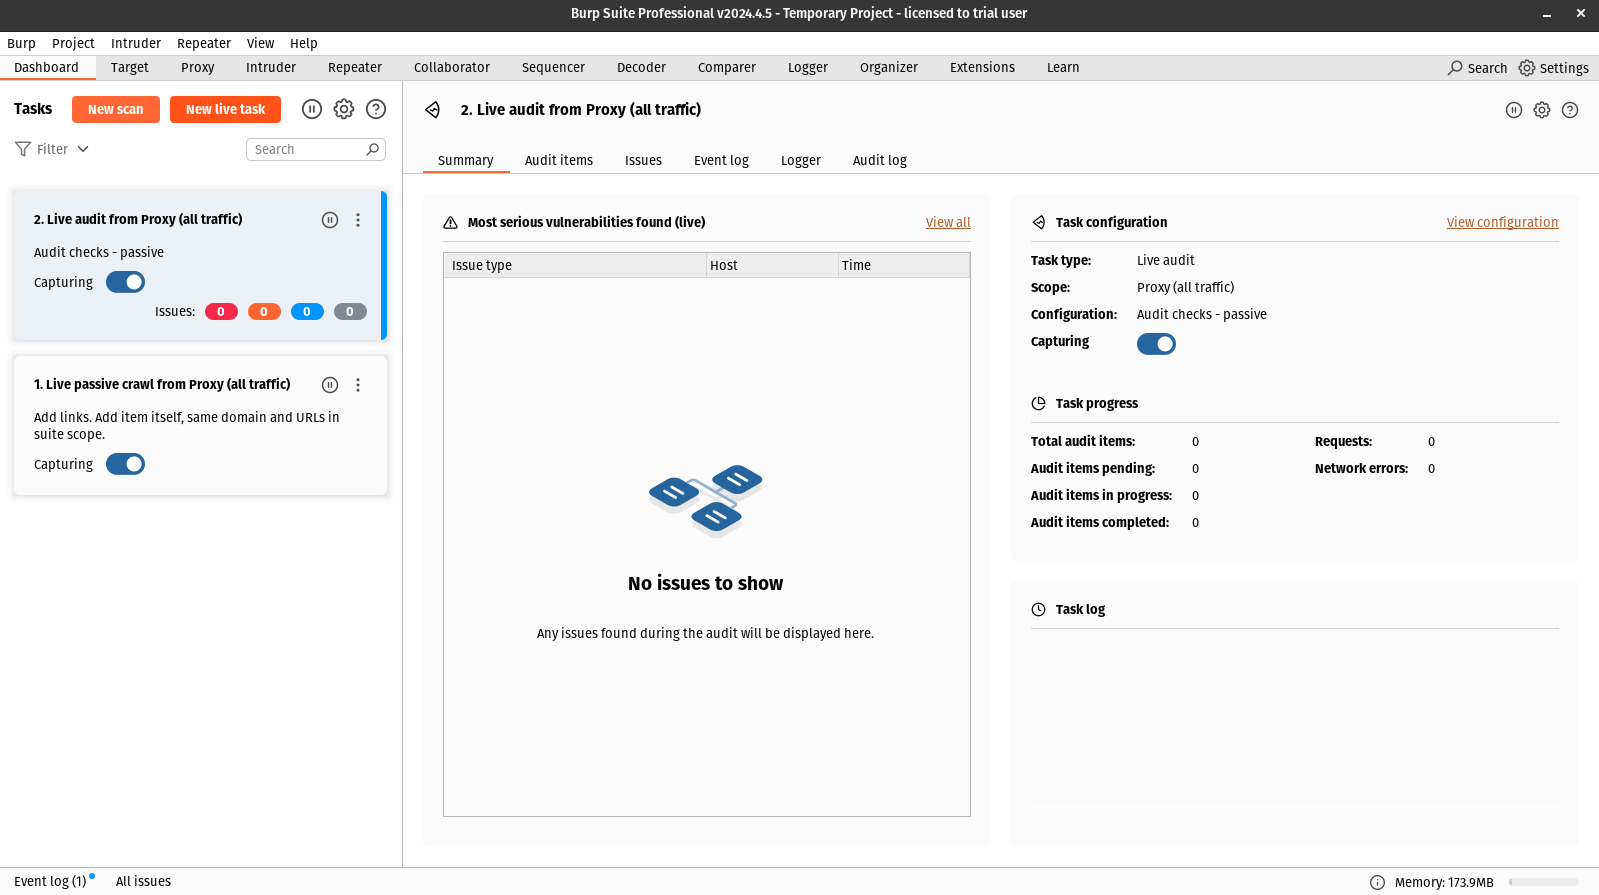
\includegraphics[width=1\textwidth]{slike/burp_start.png}
    \caption{Izgled Burp suita pri pokretanju}
    \label{slk:burp_start}
\end{figure}
\subsection{\textit{Proxy}}
Burp \textit{Proxy} je jedan od glavnih modula Burp Suitea. On omogućava presretanje, pregled i promjenu HTTP i HTTPS zahtjeva između preglednika i web aplikacije. 
Koristeći Proxy, sigurnosni stručnjaci mogu analizirati zahtjeve i odgovore, tražiti ranjivosti i manipulirati podacima kako bi testirali sigurnost web aplikacije.\cite{burp_feat}

\subsection{\textit{Intruder}}
Burp \textit{Intruder} je modul za automatizirane napade. Može se koristiti za \textit{brute force} napade, testiranje valjanosti unosa, traženje skrivenih direktorija ili datoteka, 
te druge vrste napada. Korisnik može konfigurirati različite parametre i payload-ove koji će se automatski slati, a Intruder će analizirati odgovore kako bi identificirao 
potencijalne ranjivosti.\cite{burp_feat}

\subsection{\textit{Repeater}}
\textit{Repeater} omogućava korisnicima da ponavljaju HTTP/HTTPS zahtjeve ručno. Ovo je korisno za detaljno testiranje specifičnih zahtjeva i odgovora. Korisnik može modificirati i 
ponovo poslati zahtjeve, te analizirati odgovore kako bi identificirao ranjivosti i prijetnje.\cite{burp_feat}

\subsection{\textit{Collaborator}}
\textit{Collaborator} je modul za otkrivanje server-side ranjivosti koje zahtijevaju interakciju s vanjskim sustavima/stranicama. Primjeri ovih ranjivosti uključuju 
SSRF (engl. \textit{Server-Side Request Forgery}) i različite vrste injekcija koje rezultiraju vanjskim interakcijama. Omogućava postavljanje posebnog servera koji prati 
ove interakcije i pomaže u identifikaciji ranjivosti.\cite{burp_feat}

\subsection{\textit{Comparer}}
\textit{Comparer} omogućava uspoređivanje dva skupa podataka. Ovo može biti korisno za analizu promjena između dva odgovora ili zahtjeva, kako bi se identificirale suptilne razlike koje 
mogu ukazivati na ranjivosti kao što su neodgovorna obrada zahtjeva pri kojoj mogu iscuriti informacije iz takozvanih 'sporednih kanala'. \cite{burp_feat}

\subsection{\textit{Extensions}}
\textit{Extensions} modul omogućava proširivanje funkcionalnosti Burp Suitea putem dodataka (ekstenzija). Korisnici mogu instalirati ekstenzije iz BApp Storea ili kreirati 
vlastite koristeći Burp Extender API. Ovo omogućava prilagođavanje alata specifičnim potrebama i dodavanje novih funkcija koje nisu dostupne u osnovnoj verziji.\cite{burp_feat}


\newpage
\section{Usporedba alata \textit{a priori}}
U svojoj suštini ZAP i Burp suite Professional imaju iste funkcionalnosti. Kroz godine su OWASP i nezavisni programeri polako gradili alat koji sada već može parirati profesionalnom
plaćenom alatu.
Kao što se iz tablice \ref{tbl:usporedba} zaključiti ZAP po svemu parira Burp suite-u, no i dalje oba alata imaju prednosti i mana. Jedna od većih mana Burp Professional Suita je njegova cijena gdje će nas samo jedna godina licence koštati 450 eura.
Manjkavost ZAP-a je \textit{Fuzzer}. U trenutku izrade rada funkcionalnost tog modula nije u potpunosti realizirana kao kod Burp-a što će kasnije biti pokazano.
Funkcionalnosti koje ZAP ima a Burp suite nema su mogućnost automatizacije i HUD (engl. \textit{Heads Up Display}). Automatizaciju ZAP sam prije spomenuo a HUD ću koristiti i objasniti prilikom testiranja.
Što se tiče korisničkog sučelja oba alata pružaju lijepo i moderno sučelja, gdje Burp ima malu prednost zbog jasnoće i intuitivnosti kartica i modula.
\begin{table}[H]
  \centering
  \caption{Burp suite modul i odgovarajuća alternativa realizirana u ZAP-u\cite{burp_to_zap}}
  \begin{tabular}{|c|c|}
      \hline
      \textbf{Burp Suite Professional značajka} & \textbf{ZAP alternativa} \\
      \hline
      Collaborator & OAST Support Add-on \\
      Comparer & Diff \\
      Decoder & Encoder \\
      DOM Invader & Eval Villian ekstenzija \\
      Extender & Marketplace, Scripts \\
      Intercept & Breakpoints \\
      Intruder & Fuzzer\textbf{*} \\
      Live scan & ATTACK Mode \\
      Project Files & Session Files \\
      Proxy & Proxy \\
      Repeater & Manual Request Editor, Requester ekstenzija \\
      Scanner & Active Scanner \\
      Sequencer & Token Generation and Analysis \\
      Target & Contexts \\
      \hline
  \end{tabular}
\label{tbl:usporedba}
\end{table}
% \chapter{Testiranje}
%\section{Opis testiranja}
Jedini pravi način da se objektivno usporedi efektivnost oba alata jest da ih se testira na realnim i konkretnim situacijama. Za testiranje će se koristiti Burp Suite Web Security Academy laboratorijske vježbe.\cite{burp_labs}
Osim što postoje vodiči za Burp Suite postoje i vodiči za ZAP koje su korisnici pisali.\cite{owasp_2fa_manual,owasp_b-f_manual}
Vježbe su odabrane uz pomoć OWASP Top 10 stranice\cite{owasp_top10} koja vodi brigu o broju i vrsti sigurnosnih rizika koji su do godine pisanja bili najčešći, 
te njihove povezane CWE-ove.
Obraditi će se laboratorijske vježbe povezane sa sigurnosnim rizicima s vrha gore navedenog popisa. Specifično su izabrane one za koje postoje rješenja u ZAP vodiču ili čija se rješenja mogu lako pronaći.
%%%%%%%%%%%%%%%%%%%%%%%%%%%%%%%%%%%%%%%%%%%%%%%%%%%%%%%%%%%%%%%%%%%%%%%%%%%%%%%%%%%%%%%%
%     SQL
%%%%%%%%%%%%%%%%%%%%%%%%%%%%%%%%%%%%%%%%%%%%%%%%%%%%%%%%%%%%%%%%%%%%%%%%%%%%%%%%%%%%%%%%
\section{Vidljiva pogreška bazirana na SQL injekciji}
%\subsection{Općenito}
SQL injekcije su među najčešćim prijetnjama na Internetu. Činjenica koje to dokazuje je da su s ostalim vrstama injekcija 2017.\ predstavljale najrasprostranjeniji sigurnosni rizik ,a 2021.\ su bile čak 
na trećem mjestu po učestalosti.\cite{owasp_top10}
SQL injekcija je tehnika napada u kojoj napadač ubacuje zlonamjerni SQL kod u polja za unos aplikacije kako bi izvršio neovlaštene radnje na bazi podataka. To 
može uključivati dobivanje osjetljivih podataka, izmjenu podataka, brisanje podataka ili izvođenje administrativnih operacija. 
SQL injekcija nastaje zbog neadekvatnog filtriranja ili validacije korisničkog unosa.\cite{clarke_sql,sql_w3}

Laboratorijska vježba sadrži ranjivost na SQL injekcije koju će biti iskorištena. Od ostalih informacija znamo da aplikacija koristi 'kolačiće' za analitiku te provodi SQL upit 
s informacijama u podnesenim kolačićima. Rezultati SQL se ne vraćaju direktno već je potrebno izazvati grešku u ispisu. Baza podataka sadrži tablicu zvanu \textit{users} sa stupcima \textit{username} i \textit{password}.
Cilj laboratorijske vježbe je pronalazak načina da web aplikaciji 'iscuri' lozinka za korisnika \textit{administrator} te se onda treba ulogirati s njihovim računom.

Ono što je također bitno za primjetiti je da se ne koriste podatci dobivene direktno iz malicioznog SQL upita, već grešku koja se zbog upita vraća. To uvelike otežava alatima da primjete takve ranjivosti kako \textit{de facto} nema polja koje bi mogli iskoristiti da nam aplikacija da neke djelove baze podataka direktno. 
Umjesto toga cilj je iskoristiti lošu obradu grešaka.\cite{sql_lab} 

\subsection{Vježba 1: Burp Suite}
Nakon otvaranja alata potrebno je kliknuti na karticu \textit{Target} kako je prikazano na slici \ref{slk:target_burp}.
\begin{figure}[H]
    \centering
    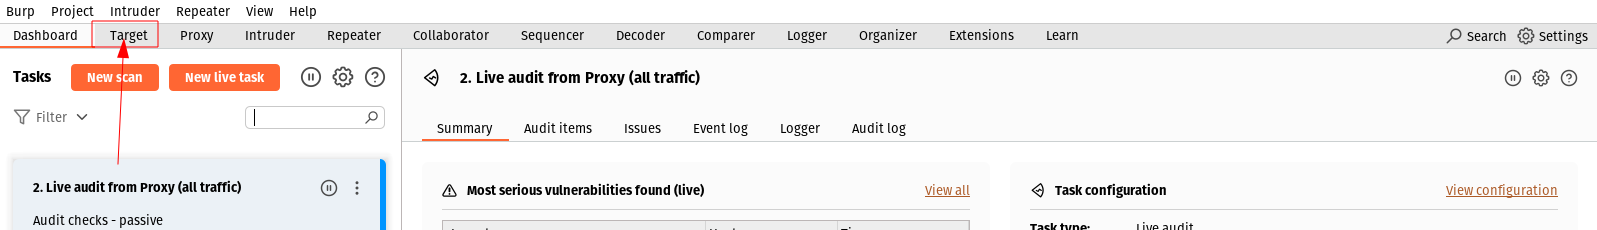
\includegraphics[width=1\textwidth]{slike/BURP_target.png}
    \caption{Popis svih kartica s naznačenom karticom \textit{Target}}
    \label{slk:target_burp}
\end{figure}

Ondje je prije svega potrebno uključiti proxy koji će biti korišten za presretanje zahtjeva i odgovora. Zatim je potrebno kliknuti na gumb \textit{Open browser} te u adresnu traku zalijepiti adresu laboratorijske
vježbe. Odmah prilikom otvaranja dediciranog pretraživača i unosom poveznice na vježbu Burp izgradi \textit{sitemap} (mapu cijele stranice).
Sada kako bi bilo moguće pronaći ranjivost koja će se iskoristiti za navedenu vježbu nužno je započeti skeniranje s kartice \textit{Dashboard > New scan > Webapp scan}.
Najprije se prikazuje pregled skena kao što je vidljivo na slici \ref{slk:burp_pojed}. Ovdje se mogu vidjeti generalne informacije o meti i trenutnim postavkama skena.
Potom se konfigurira sken kao što je to vidljivo na slici \ref{slk:burp_config}. Prilikom ove i budućih vježbi koristiti će se \textit{Deep} sken.
\begin{figure}[H]
    \centering
    \begin{minipage}[b]{0.46\textwidth}
      \centering
      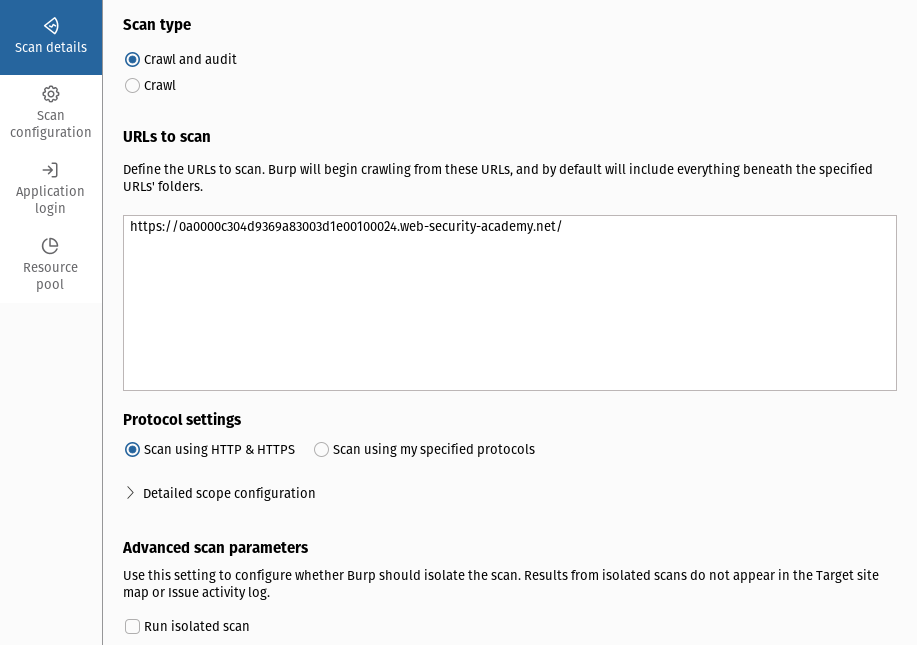
\includegraphics[width=\textwidth]{slike/scan_det.png}
      \caption{Pojedinosti skena}
      \label{slk:burp_pojed}
    \end{minipage}
    \hspace{0.05\textwidth} % Razmak između slika
    \begin{minipage}[b]{0.47\textwidth}
      \centering
      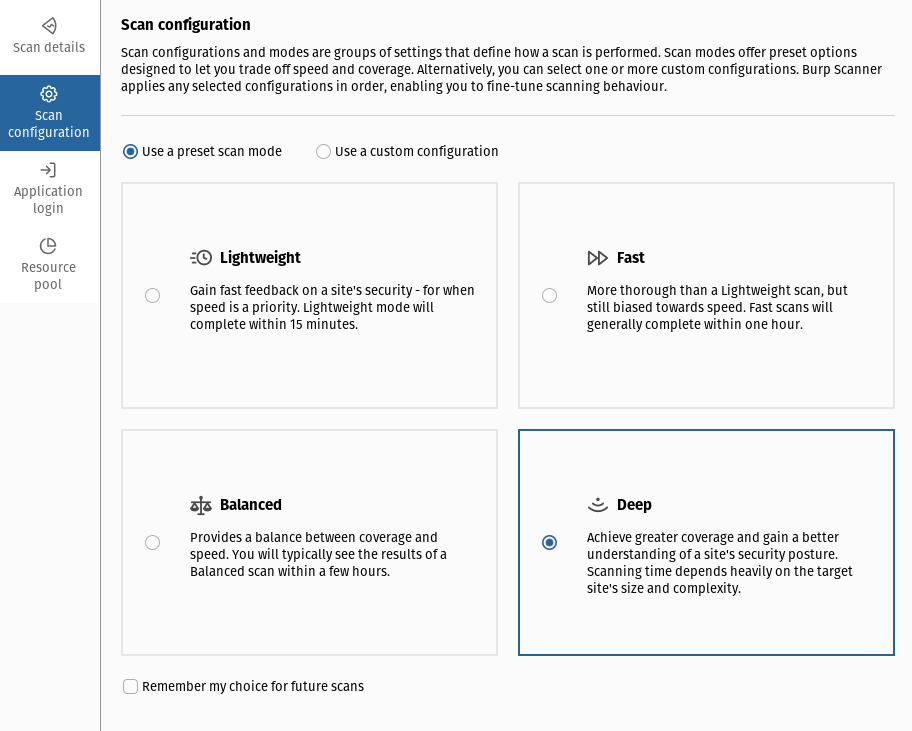
\includegraphics[width=\textwidth]{slike/scan_config_burp.png}
      \caption{Konfiguriranje skena}
      \label{slk:burp_config}
    \end{minipage}
  \end{figure}

\lstset{language=SQL}
Skeniranje traje <5 minuta te izvodi očekivane rezultate. Osim SQL ranjivosti, alat je pronašao nekolicinu informativnih detalja što se stranice tiče poput činjenice da komunikacija nije enkriptirana 
te kako nije definirana striktna sigurnosna politika za transport.
Vezano za SQL injection alat je pronašao ranjivosti na čak 3 putanje \textit{/product, /filter} i \textit{/my-account}. Za product i filter je koristio \textit{payload} u kojem je u
\textit{trackingid} prvo dodao jednu ' a nakon što je aplikacija javila grešku dodao '' na kraj \textit{TrackingId}-a nakon koje je greška nestala. Zatim je pokušao napraviti novi payload viljiv na slici \ref{slk:burp_auto}
nakon čega je primijetio da stranici treba dulje da odgovori te je deducirao da se najvjerojatnije radi o Postgres bazi podataka. Sa slike je vidljivo kako je iskorištena naredba za spavanje integrirana kao dio \textit{TrackingId}-a koju 
baza nakon parsiranja izvršava.

\begin{figure}[h]
  \centering
  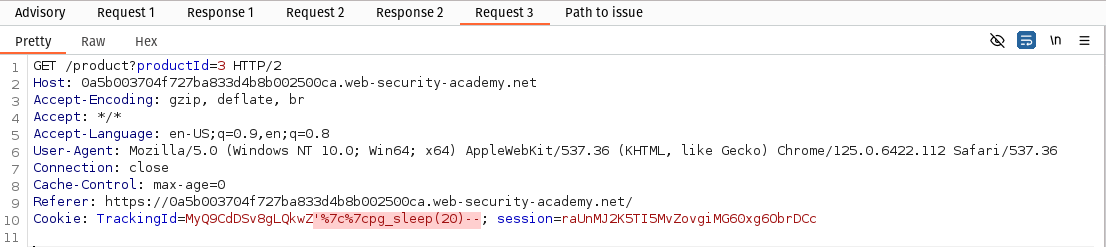
\includegraphics[width=1\textwidth]{slike/sql_requests.png}
  \caption{Zahtjev koji je otkrio bazu podataka i iskoristio SQL ranjivost}
  \label{slk:burp_auto}
\end{figure}

Pod karticom \textit{Advisory} s slike \ref{slk:burp_auto} je vidjljivo koji CWE se krije iza otkrivene ranjivosti te detalje o ispitanoj ranjivosti. Sada je potrebno iskoristiti ovo znanje prilikom napada web aplikacije te potom izvršiti prijavu kao \textit{administrator}.
Prvo se navigira u karticu \textit{Proxy > HTTP history}. Ondje se nalazi GET zahtjev za putanju \textit{/login} te je potrebno modificirati dio kolačića gdje piše \textit{TrackingId} tako da na kraj vrijednosti stoji '.
To će natjerati stranicu da izbaci pogrešku iz kojeg se otkriva cijeli SQL upit što je vidljivo na slici \ref{slk:err_test}.

\begin{figure}[]
    \begin{lstlisting}[frame=single, breaklines]
        Unterminated string literal started at position 52 in SQL SELECT * FROM tracking WHERE id = 'JhlbaDuQVof0JeOw''. Expected char
    \end{lstlisting}
    \caption{Dobivena pogreška}
    \label{slk:err_test}
\end{figure}

Sada je potrebno modificirati taj zahtjev kako bi došli do lozinke korisnika \textit{administrator}. Dobar bi pokušaj bio potpuno maknuti vrijednost \textit{TrackingId} argumenta i zamijeniti ju sa zloćudnim SQL upitom.
Koristeći Repeater modul (desni klik na zahtjev > \textit{Send to Repeater}) te ćemo ondje izmijeniti vrijednost tako da sad u payload-u piše: \newline
\textit{TrackingId=' AND 1=CAST((SELECT username FROM users LIMIT 1) AS int)--}

Iz prijašnje greške \ref{slk:err_test} može se zaključiti da aplikacija traži samo jedan \textit{TrackingId} te da je vjerojatno potrebno ograničiti upit na jedan redak baze kao i jedan stupac.
Sada bi trebala doći nova greška koja kaže kako \textit{administrator} nije tipa \textit{integer}. Iz ove greške je očito da se administrator nalazi prvi na popisu. Kao što je vidljivo potrebno je pretvoriti polja koja nisu \textit{integeri} u \textit{int} upravo kako bi 
natjerali bazu da "procuri informacije".
Ponovno ćemo se sada vratiti u \textit{Repeater} te ponoviti prijašnji zahtjev s malom preinakom:\newline
\textit{TrackingId=' AND 1=CAST((SELECT password FROM users LIMIT 1) AS int)--}

Ovaj upit napokon otkriva password za korisnika \textit{administrator} \ref{slk:err_good} no kao grešku.
\begin{figure}[H]
    \begin{lstlisting}[frame=single, breaklines]
        ERROR: invalid input syntax for type integer: "vuapcoxchp374pzq5d31"
    \end{lstlisting}
    \caption{Pogreška koja ispisuje lozinku za administratora}
    \label{slk:err_good}
\end{figure}
\newpage % dodano radi urednosti
\subsection{Vježba 1: ZAP}
Najprije u gornjem desnom kutu alat je potrebno postaviti \textit{Mode} na ATTACK. Zatim je potrebno kliknuti na \textit{Automated scan} i unijeti link mete.
Skeniranje traje nešto dulje od Burpovog. Među alertima je vidljivo da ZAP nije primijetio da uopće postoji mogućnost SQL injection-a\ref{slk:zap_vuln}. Prije je spomenuto kako ZAP ima Fuzzer ali nije trenutno funkcionalan. Razlog tomu je što ZAP trenutno nema mogućnost 
skeniranja HTTP zaglavlja što je veliki minus u odnosu na Burp.\cite{burp_to_zap} Ovaj zadatak služi otkrivanju ove velike manjkavosti ZAP-a nad Burpom.
\begin{figure}[H]
    \centering
    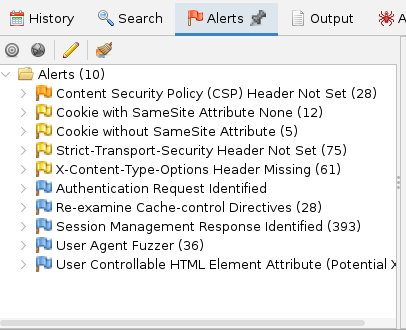
\includegraphics[width=0.8\textwidth]{slike/zap_sql_alerts.png}
    \caption{Manjak upozorenja na ranjivosti web aplikacije}
    \label{slk:zap_vuln}
\end{figure}

Problem je moguće zaobići koristeći ZAP HUD.\@ To je modul koji omogućava ručnu provjeru, izmjenu i slanje zahtjeva. Nakon što se uključi \textit{Break} prilikom gledanja \textit{/login} putanje nakon klika na gumb Login.
Ovdje je potrebno izmijeniti HTTP zaglavlje te modificirati kolačić kao što je prethodno to učinjeno za Burp. Naravno sada je otkriveno dobro rješenje na isti način kao i za Burp.
%%%%%%%%%%%%%%%%%%%%%%%%%%%%%%%%%%%%%%%%%%%%%%%%%%%%%%%%%%%%%%%%%%%%%%%%%%%%%%%%%%%%%%%%
%     2FA
%%%%%%%%%%%%%%%%%%%%%%%%%%%%%%%%%%%%%%%%%%%%%%%%%%%%%%%%%%%%%%%%%%%%%%%%%%%%%%%%%%%%%%%%
\newpage % dodano radi urednosti
\section{Dvofaktorska autentifikacija sa pogrešno konfiguriranom logikom}
%\subsection{Općenito}
Dvofaktorska autentifikacija (2FA) je sigurnosni mehanizam koji koristi dva različita faktora za provjeru identiteta korisnika, kao što 
su lozinka (prvi faktor) i jednokratni kod poslan putem SMS-a ili aplikacije (drugi faktor). Iako 2FA značajno povećava sigurnost, može 
biti ranjiv na određene vrste napada ako nije pravilno implementiran.\cite{dmitrienko2014security,aloul2009two}
Primjeri loše implementacije su recikliranje sigurnosnih kodova, realizacija 2FA na klijentskoj strani, direktan pristup API-ju, loša programska potpora i mnogi drugi.

Ova laboratorijska vježba ima ranjivost u dvofaktorskoj autentifikaciji zbog pogrešne logike, konkretno uz zahtjev za unos sigurnosnog koda u kolačiću prenosi i ime korisnika te nema limit na slanje zahtjeva što uvelike kompromitira aplikaciju.
Za rješavanje zadataka, potrebno je pristupiti računu korisnika \textit{Carlosa}.
Kao informacije za vježbu su pruženi podatci za pristup korisniku \textit{wiener} s lozinkom \textit{peter} te pristup mail serveru.\cite{2FA_lab}
Također je dan hint kako se korisnik \textit{carlos} neće pokušati ulogirati za vrijeme trajanja napada.

\subsection{Testiranje: Burp Suite}
Skeniranje se pokreće kao u prethodnoj vježbi. 
Kao u stvarnim situacijama, zanimljivi su POST zahtjevi koje skener šalje. 
Pokušat će se iskoristiti \textit{/login} putanja za rješavanje vježbe. 
Prije svega, pokušava se ulogirati s danim vjerodajnicama, nakon čega se traži unos 4-znamenkastog koda koji je poslan na mail. 
Već sada se uočava manjkavost realizacije. 
Ako kod ima samo 4 znamenke, to znači da postoji samo 10,000 mogućih kombinacija što nije puno za današnje sustave. 
Nakon što se uspije, pretražit će se povijest skeniranja da se vidi kako se zahtjev može izmijeniti.

Zahtjev sa putanjom \textit{/login2} šalje se na \textit{Intruder} kao što je vidljivo na slici \ref{slk:burp_req}. 
Jednom kada se uđe u Intruder, vrijednost \textit{verify} iz \textit{wiener} mijenja se u \textit{carlos} za GET zahtjev, što generira privremeni kod. 
Zatim se POST zahtjev iste putanje šalje na Intruder te se bira način rada \textit{Sniper} i označava vrijednost polja \textit{mfa-code} za modificirani payload što je vidljivo na \ref{slk:burp_req_config}. 
Burp će sada slati zahtjeve, svaki put modificirajući payload, kako bi pogodio točan kod za carlosa.

\begin{figure}[H]
  \centering
  \begin{minipage}[b]{0.45\textwidth}
    \centering
    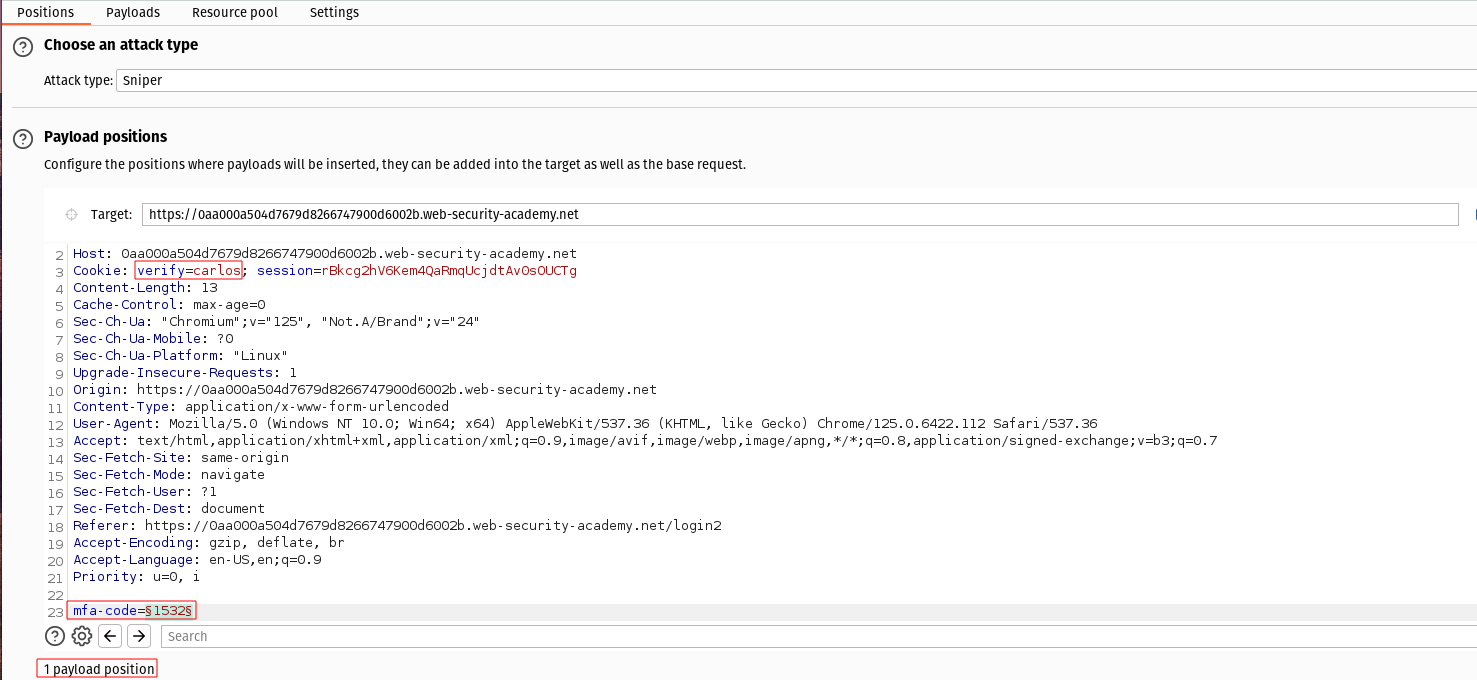
\includegraphics[width=\textwidth]{slike/intruder_2fa.png}
    \caption{Zahtjev koji ćemo koristiti u Intruderu}
    \label{slk:burp_req}
  \end{minipage}
  \hspace{0.05\textwidth} % Razmak između slika
  \begin{minipage}[b]{0.45\textwidth}
    \centering
    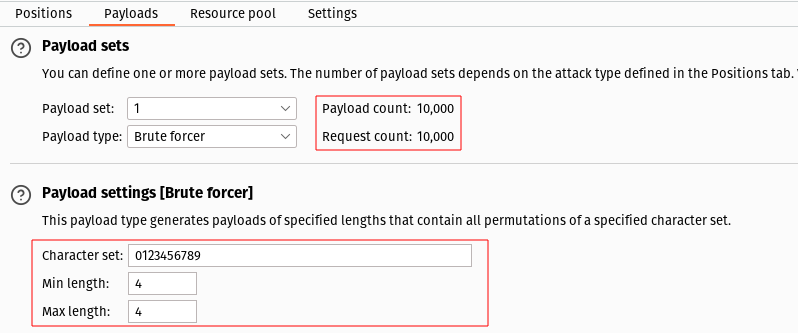
\includegraphics[width=\textwidth]{slike/payload_intruder.png}
    \caption{Konfiguriranje payloada}
  \end{minipage}
  \label{slk:burp_req_config}
\end{figure}

Sada se traži odgovor koji se razlikuje od drugih ili po duljini ili po vrsti odgovora. U ovom slučaju razlikovat će se i po vrsti i po duljini odgovora\ref{slk:burp_atks}. Jedan jedini payload vratio se s odgovorom 302, što označava redirekciju. Kada se pogleda vrijednost payloada za taj zahtjev, vidi se da je Carlosov trenutačni kod 0100.
\begin{figure}[H]
  \centering
  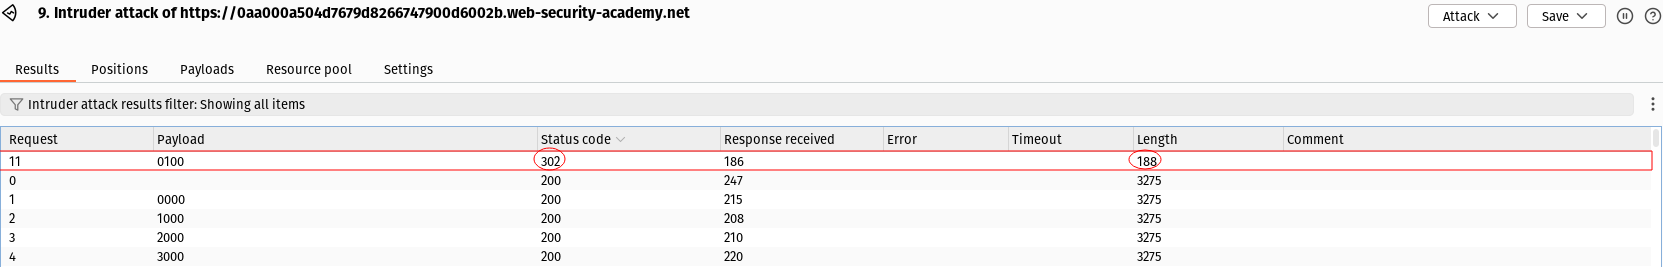
\includegraphics[width=1\textwidth]{slike/intruder_atk.png}
  \caption{Prikaz napada uz modul Intruder}
  \label{slk:burp_atks}
\end{figure}

Odgovor se učita u pretraživač ili se kod ručno unese, čime se završava vježba. Pritom se mora paziti da se na preostalim zahtjevima za vrijednost \textit{verify} upiše \textit{carlos}.\newpage % dodano radi urednosti

\subsection{Testiranje: ZAP}
Kako je već mnogo poznato o web aplikaciji, testiranje se može brže provesti. Sa ZAP HUD-om se ponovno normalno ulogira kao što je to učinjeno kod Burpa. Nakon što se ulogira s danim vjerodajnicama, otići će se u karticu \textit{History} u glavnom izborniku. Ondje se izabire GET zahtjev za \textit{/login2} putanju, te mu se modificira vrijednost \textit{verify} i zahtjev se šalje.

Zatim se pronađe stari POST zahtjev za \textit{/login2}. Kako generator regularnih izraza nije funkcionalan u ZAP-u, potrebno je napraviti kratki "obilazak". Prvo se dodaje generator zahtjeva tipa \textit{Numberzz}, koji stvara brojeve od 0 do 9999 što je vidljivo na slici \ref{slk:zap_gen}. Nakon toga je iz slike \ref{slk:zap_config_proc} vidljivo da je potrebno namjestiti procesor za zahtjeve koji će zahtjeve pretvoriti u oblik koji je zapravo potreban.
\begin{figure}[H]
  \centering
  \begin{minipage}[b]{0.5\textwidth}
    \centering
    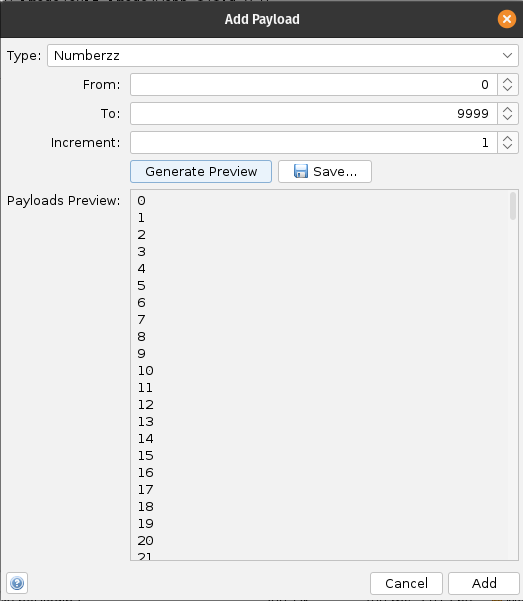
\includegraphics[width=\textwidth]{slike/payload_fuzz.png}
    \caption{Dodavanje generatora}
    \label{slk:zap_gen}
  \end{minipage}
  \hspace{0.05\textwidth} % Razmak između slika
  \begin{minipage}[b]{0.4\textwidth}
    \centering
    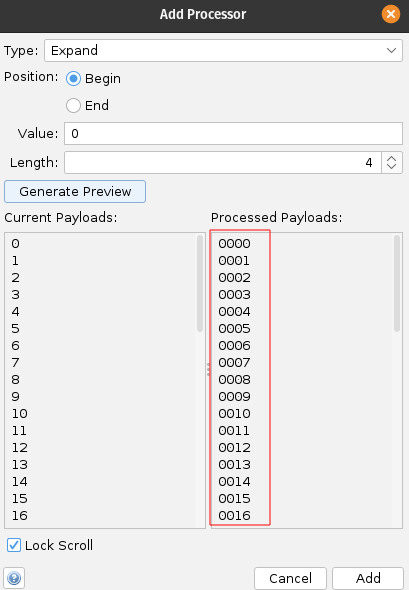
\includegraphics[width=\textwidth]{slike/processor_fuzz.png}
    \caption{Konfiguriranje procesora zahtjeva}
    \label{slk:zap_config_proc}
  \end{minipage}
\end{figure}

Kao i u radu s Burpom sada se pronalazi odgovor koji se razlikuje te se šalje pregledniku. Nakon toga bi se trebalo pojaviti na zaslonu nešto kao na slici \ref{slk:zap_succ}.

\begin{figure}[H]
  \centering
  
\includegraphics[width=0.4\textwidth]{slike/2fa_succ.png}
  \caption{Prikaz uspješne prijave}
  \label{slk:zap_succ}
\end{figure}
%%%%%%%%%%%%%%%%%%%%%%%%%%%%%%%%%%%%%%%%%%%%%%%%%%%%%%%%%%%%%%%%%%%%%%%%%%%%%%%%%%%%%%%%
%     Brute force
%%%%%%%%%%%%%%%%%%%%%%%%%%%%%%%%%%%%%%%%%%%%%%%%%%%%%%%%%%%%%%%%%%%%%%%%%%%%%%%%%%%%%%%%
\section{Napad silom na lozinku koristeći lošu implementaciju promjene lozinke}
Napad grubom silom na lozinku podrazumijeva isprobavanje svih mogućih kombinacija dok se ne pronađe točna. 
Kada se kombinira s loše implementiranom funkcionalnošću promjene lozinke, mogu se pojaviti ozbiljni sigurnosni problemi. 
Primjerice, ako sustav dopušta korisniku da promijeni lozinku bez provjere identiteta putem adekvatnih metoda (npr. slanje privremene lozinke na unaprijed spremljeni mail, korištenje dvofaktorske autentifikacije), otvara se prostor za iskorištavanje ranjivosti.
U takvim scenarijima, napadač koji dobije pristup korisničkom računu putem metoda poput napada grubom silom ili socijalnog inženjeringa može lako promijeniti lozinku i time zaključati legitimnog korisnika. 
To se događa jer sustav ne provjerava dovoljno identitet korisnika prije nego što dopusti promjenu lozinke.

Kako bi se smanjili rizici, ključno je implementirati robustne sigurnosne mjere poput dvofaktorske autentifikacije, obavijesti o promjeni lozinke na registrirani virtualni sandučić (engl. \textit{mail}), specifične fraze koje se generiraju za svakog korisnika pri registraciji i slična rješenja.
Nažalost, napade grubom silom je gotovo nemoguće spriječiti te bi dizajneri trebali ciljati na to da je ovo najbolji mogući napad koji se pruža napadačima jer je ekstenzivan te u puno slučajeva zahtjeva puno vremena i resursa.\cite{knudsen2011brute} 

Sigurnosni propust u funkcionalnosti promjene lozinke u ovoj laboratorijskoj vježbi čini ju podložnom napadima grubom silom. Za rješavanje ove vježbe, potrebno je iskoristiti listu potencijalnih lozinki kako bi se pristupilo Carlosovom korisničkom računu. 
Informacije koje su na raspolaganju uključuju vlastite vjerodajnice (wiener:peter), korisničko ime \textit{carlos}, te listu kandidata za lozinku u obliku teksta gdje je svaka potencijalna lozinka zapisana u zaseban redak.\cite{brute_lab}
\newpage %dodano radi preglednosti
\subsection{Testiranje: ZAP}
Prije nego što se započne s ručnim testiranjem aplikacije, provest će se automatizirani sken kako bi se dobila mapa povezanih stranica (engl. \textit{sitemap}). 
Iako neće puno pomoći u rješavanju ove konkretne vježbe, uvijek je dobra praksa ispitati površinu napada kako bi se mogao pronaći dobar vektor napada. 
Sken sam po sebi ne otkriva previše, tako da će se pristupiti ručnom testiranju aplikacije uz pomoć ZAP HUD-a.

Prva stvar koja će se napraviti je prijava s danim vjerodajnicama kako bi se vidjelo kako aplikacija gradi zahtjeve za prijavu. 
Za to će poslužiti modul \textit{Break}, koji omogućuje pregled i uređivanje svakog zahtjeva prije nego što ga preglednik pošalje i odgovora prije nego što ga preglednik primi. 
Iako naslov vježbe sugerira da vjerojatno neće biti moguće iskoristiti funkcionalnost prijave, dobro je biti temeljit i vidjeti postoji li neka ranjivost koja nije namjerno ostavljena. 
U ovom konkretnom slučaju, prijava je dobro implementirana, te će se nastaviti s testiranjem. 
Sada je zaslon nakon prijave nešto drukčiji nego na prijašnjim vježbama kao što je vidljivo na slici \ref{slk:succ_login}. Vidljivo je da je osim unosa maila moguća i promjena lozinke ukoliko je poznata trenutna.
\begin{figure}[H]
  \centering
  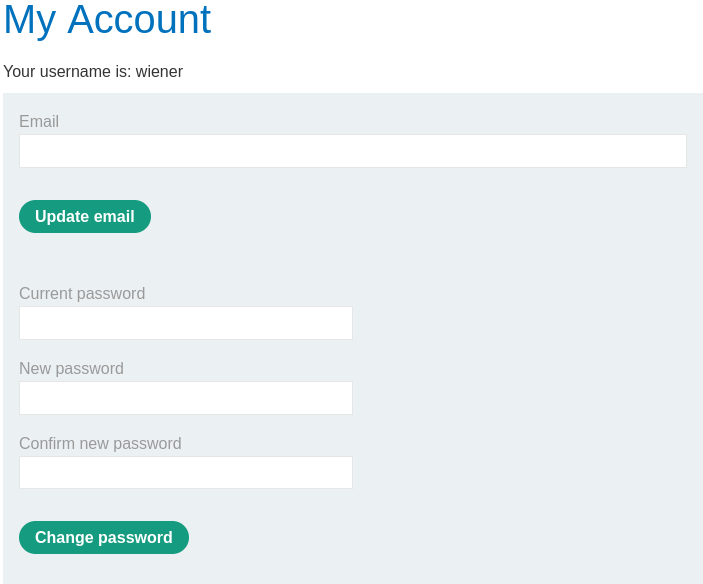
\includegraphics[width=0.6\textwidth]{slike/b_f_postLogin.png}
  \caption{Sučelje nakon prijave sa dostupnim vjerodajnicama}
  \label{slk:succ_login}
\end{figure}

Očito je da se mora dokučiti kako iskoristiti opcije za mijenjanje lozinke. 
Pokušat će se promijeniti lozinka računu kojem se ima pristup kako bi se vidjelo kako web aplikacija gradi zahtjev. 
Ponovno će se koristiti \textit{Break} funkcionalnost kako bi se presreo i uredio zahtjev vidljiv na slici \ref{slk:gen_req}. 
Označeno je tijelo zahtjeva koje je potrebno urediti.

\begin{figure}[H]
  \centering
  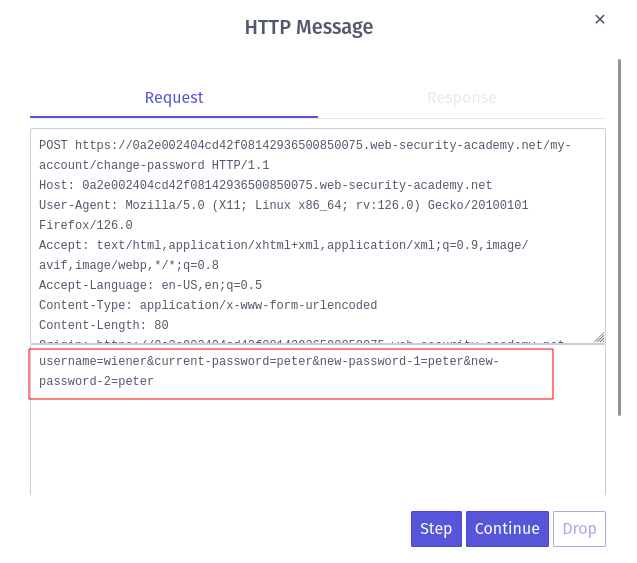
\includegraphics[width=0.8\textwidth]{slike/break_np.png}
  \caption{Zahtjev koji aplikacija generira}
  \label{slk:gen_req}
\end{figure}

Iz slike \ref{slk:gen_req} je vidljivo da se, kao u prijašnjim vježbama, može mijenjati korisničko ime kao i pripadajuća lozinka. 
Sada, kada su te putanje spremljene, koristit će se \textit{Fuzzer} kako bi se razotkrila lozinka za korisnika \textit{carlos}. 
Kako izmjena lozinki zapravo nije moguća, potrebno je na drugi način dokučiti koja je lozinka točna.
Relevantni POST zahtjev šalje se u \textit{Fuzzer}. 
Unutar \textit{Fuzzer}a korisničko ime \textit{wiener} zamjenjuje se s \textit{carlos}, a trenutna lozinka označava se kao mjesto na kojem će alat pogađati lozinke. 
Također, alat se opskrbljuje kandidatima za lozinku koji su dobiveni na početku vježbe, te se postavljaju različite nove lozinke. 
To se radi kako bi se umjesto pogreške da je lozinka netočna dobio odgovor koji javlja da se nove lozinke ne poklapaju. 
Primjer tako definiranog zahtjeva možemo vidjeti na slici \ref{slk:full_config_fuzz_zap}

\begin{figure}[H]
  \centering
  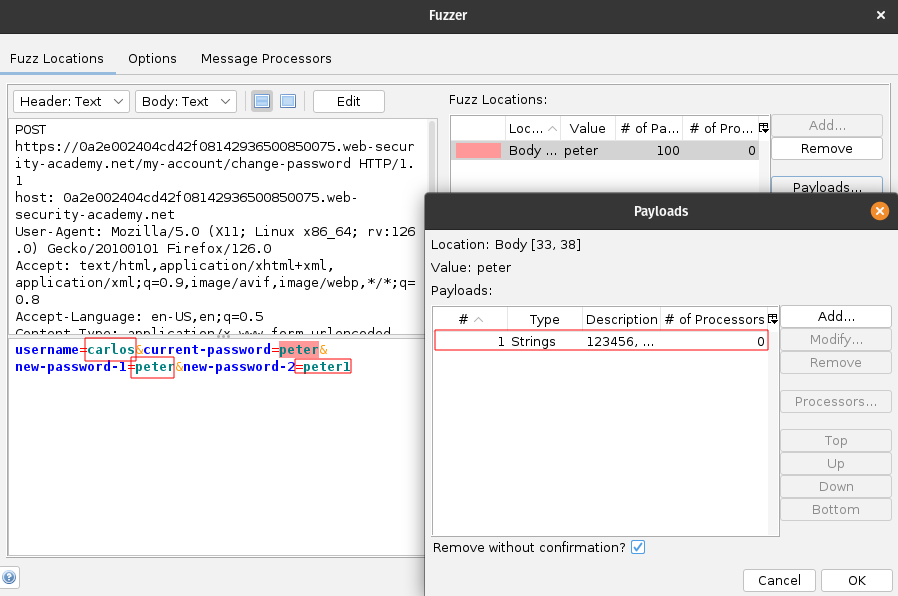
\includegraphics[width=1\textwidth]{slike/zap_fuzz_pass.png}
  \caption{Ispravno konfiguriran \textit{Fuzzer}}
  \label{slk:full_config_fuzz_zap}
\end{figure}

Sada se traži odgovor koji, među onima kojima su zaprimljeni ima različitu duljinu odgovora. 
Uz njega nam piše i koju je lozinku alat pokušao poslati. 
Sada je potrebno tu lozinku iskoristiti da za prijavu kao \textit{carlos} i tako završava ova laboratorijska vježba.

\newpage %dodano radi preglednosti
\subsection{Testiranje: Burp Suite}
Kao i za ZAP, aplikacija će se prvo skenirati kako bi se utvrdila površina napada. 
Kao i kod ZAP-a, skener nije utvrdio nikakve probleme. 
Unese se ispravna trenutna lozinka i dvije nove lozinke koje se ne podudaraju. 
Ovaj zahtjev POST /my-account/change-password šalje se u Burp Intruderu. 
Zbog prijašnjeg testiranja, zna se da je potrebno pratiti razlike u odgovorima.
U Burp Intruderu parametar username mijenja se u carlos i dodaje se položaj za promjenu za parametar trenutne lozinke. 
Provjerava se da su parametri za nove lozinke postavljeni na dvije različite vrijednosti. 
Na kartici \textit{Payloads} unosi se lista lozinki.
Kada je napad završen, može se primijetiti da je jedan odgovor drukčije duljine i sadrži poruku "Nove lozinke se ne podudaraju". 
Lozinka koja je iskorištena u tom zahtjevu je lozinka za račun \textit{carlos} što je vidljivo na slici \ref{slk:atk_end}.

\begin{figure}[H]
  \centering
  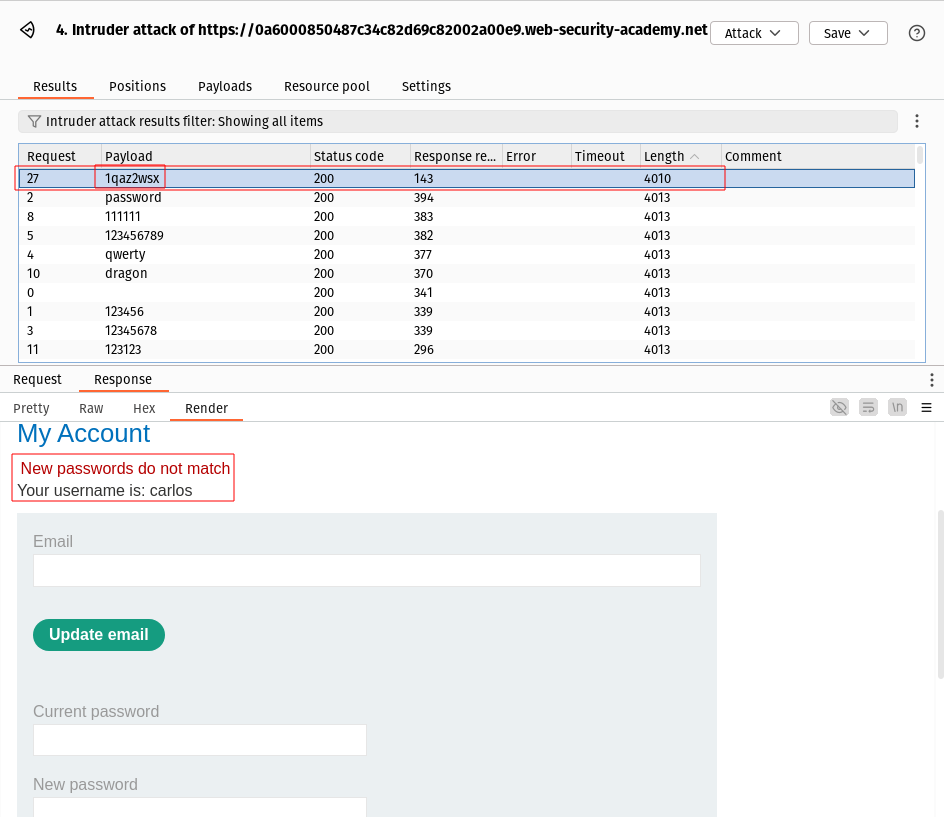
\includegraphics[width=1\textwidth]{slike/butp_bf_fuzz.png}
  \caption{Kraj napada u \textit{Intruder}u}
  \label{slk:atk_end}
\end{figure}
Rješenje u ovom slučaju je \textbf{1qaz2wsx} što je i vidljivo iz slike \ref{slk:atk_end}.
% \chapter{Usporedba i nadomještanje funkcionalnosti}
%\addcontentsline{toc}{chapter}{Usporedba i nadomještanje funkcionalnosti}
Oba alata imaju slične funkcionalnosti i mogu postići iste rezultate s minimalno različitim pristupom. 
ZAP je očito namijenjen za male tvrtke i pojedince, dok je Burp Suite komercijalan alat namijenjen za velike tvrtke i korporacije. 
Iako i velike tvrtke mogu koristiti ZAP, njihovi sigurnosni specijalisti moraju proći više obuke.

Razlike u korištenju su primijećene prilikom korištenja oba alata. 
Kada se pojavi problem s Burpom ili je potrebna informacija o njihovim alatima, uvijek se može osloniti na dobro napisanu dokumentaciju. 
\textit{PortSwigger} (tvrtka koja je izgradila Burp Suite) osigurava profesionalne priručnike i video upute za korištenje svojih alata.

Kada se pojavi problem sa ZAP-om, uvelike se oslanja na rješenja koja su već dokumentirali članovi zajednice. 
Iako ZAP ima svoje priručnike i dokumentaciju, oni nisu na razini jasnoće, pokrivenosti i razumljivosti kao Burpova dokumentacija. 
Velika prednost ZAP-a je njegov HUD, koji je bio izuzetno koristan prilikom testiranja. 
U prednost ZAP-u također idu i dodaci, tj. ekstenzije, kojih ima puno više nego za Burp. 
Te ekstenzije mogu se pisati u \textit{Javi, Pythonu, Rubyu, JavaScriptu}, itd. 
Osim toga, ZAP je moguće uključiti u skripte te na taj način automatizirati testiranje.

Primjer takve skripte:

\captionsetup[figure]{labelformat=empty, labelsep=none}

\begin{figure}[H]
    \begin{verbatim}
    import time
    from zapv2 import ZAPv2

    def zap_scan(target_url, api_key='vas_api_kljuc', log='zap_rezultati.txt'):
        zap = ZAPv2(apikey=api_key)
        zap.urlopen(target_url)
        time.sleep(2)
        zap.spider.scan(target_url)
        while int(zap.spider.status('')) < 100:
            time.sleep(2)
        zap.ascan.scan(target_url)
        while int(zap.ascan.status('')) < 100:
            time.sleep(5)
        alerts = zap.core.alerts() # rjecnik alarma
        with open(log, 'w') as f:
            for alert in alerts:
                f.write(f"Alert: {alert['alert']}\nRisk: {alert['risk']}\n \
                URL: {alert['url']}\n Description: {alert['description']}\n \
                Solution: {alert['solution']}\nReference: {alert['reference']}\n)

    if __name__ == "__main__":
        target_url = input("Unesite URL zrtve: ")
        zap_scan(target_url)
    \end{verbatim}
    \captionsetup{labelformat=empty} % To remove the default "Figure" label
    \caption{\textbf{Ispis 3.18.} Jednostavna skripta za automatizaciju skeniranja u Pythonu\cite{zap_script}}
    \label{inp:script}
\end{figure}

Jedino što je potrebno napraviti je instalirati ZAP i Python, postaviti api ključ za korištenje, pokrenuti ZAP u \textit{daemon} načinu rada
te onda sa Pythonovim menadžerom za pakete instalirati paket za korištenje ZAP daemona.

\noindent
\texttt{./zap.sh -daemon -config api.key=your\_api\_key}\newline
\texttt{pip install python-owasp-zap-v2.4}
% \chapter{Zaključak}
Ovaj rad dokazuje da OWASP ZAP može poslužiti kao adekvatna zamjena za Burp Suite Professional u mnogim aspektima 
testiranja sigurnosti web aplikacija. Provedena testiranja na konkretnim laboratorijskim vježbama pokazala su da oba alata mogu 
detektirati i iskoristiti iste ranjivosti, iako ponekad različitim pristupima.
ZAP se istaknuo svojim intuitivnim sučeljem, posebice HUD-om koji olakšava interaktivno testiranje. 
Također, njegova otvorenost za proširenja i mogućnost automatizacije putem skripti čine ga izuzetno fleksibilnim alatom. 
S druge strane, Burp Suite Professional nudi nešto sofisticiraniji skup alata i bolje dokumentiranu podršku, što ga čini preferiranim 
izborom za veće organizacije i profesionalne penetracijske testere.

Ipak, postoje određene funkcionalnosti u kojima ZAP zaostaje, poput nemogućnosti skeniranja HTTP headera, što je bilo vidljivo u vježbi 
s SQL injekcijom. No, takvi nedostaci često se mogu nadomjestiti korištenjem dodataka ili alternativnih metoda.
Ključna prednost ZAP-a je svakako njegova dostupnost kao besplatnog alata otvorenog koda, što ga čini pristupačnim pojedincima i manjim 
timovima koji si ne mogu priuštiti skupe licence. Uz to, aktivna zajednica koja stoji iza ZAP-a kontinuirano radi na poboljšanjima i  
proširenjima, čime se ovaj alat neprestano unapređuje.

Zaključno, iako Burp Suite Professional i dalje drži vodeću poziciju na tržištu, OWASP ZAP se pokazao kao snažan i sposoban alat koji 
može zadovoljiti većinu potreba u području testiranja sigurnosti web aplikacija. Izbor između ova dva alata često će ovisiti o 
specifičnim potrebama projekta, raspoloživom budžetu i stručnosti tima. U svakom slučaju, postojanje kvalitetne besplatne alternative 
poput ZAP-a značajno decentralizira tržište alatima za kibernetičku sigurnost, što u konačnici doprinosi sigurnijem web okruženju te 
osigurava nadmetanje i konstantnu inovaciju.
%\bibliography{literatura}
\chapter{Uvod i evolucija tehnologija}

Sigurnosni krajolik kontinuirano evoluira od tradicionalnih IDS/NIDS sustava prema sofisticiranim XDR platformama. Ova evolucija reflektira rastuće potrebe organizacija za proaktivnim, automatiziranim i sveobuhvatnim sigurnosnim rješenjima.

Progresivni razvoj može se prikazati kroz četiri glavne ere. IDS/NIDS era karakterizirana je pasivnom detekcijom i uzbunijavanjem, EDR era donosi fokusirane endpoint response capabilities, NDR era uvodi mrežno-centriranu detekciju i response, dok XDR era predstavlja holističku integraciju svih sigurnosnih slojeva. Matematički odnos $(NDR \cup EDR) \subset XDR$ potvrđuje da XDR predstavlja superset postojećih tehnologija, a ne njihovu zamjenu.

\chapter{Komparativna analiza osnovnih alata}

\section{IDS i NIDS sustavi}

IDS (Intrusion Detection System) predstavlja temeljnu sigurnosnu tehnologiju za skeniranje sustava i detekciju upada, dok je NIDS (Network Intrusion Detection System) specijalizirana varijanta fokusirana na mrežni promet. Osnovna razlika između IDS/NIDS i DR sustava leži u tome što IDS sustavi pružaju pasivno nadgledanje i uzbunjivanje, dok DR sustavi omogućavaju aktivno nadgledanje s mogućnostima automatskog odgovora poput izolacije kompromitiranih uređaja i blokiranja sumljive komunikacije.

Snort je jedan od najpoznatijih open-source IDS/IPS alata s pravilima zasnovanim na prepoznavanju uzoraka. Pogodan je za manje mreže ali može biti ograničen kod velikih mrežnih opterećenja zbog single-threaded arhitekture. Suricata predstavlja napredni IDS/IPS alat s paralelnom obradom paketa što rezultira boljim performansama od Snorta. Kompatibilan je sa Snort pravilima i ima naprednije mogućnosti za veliku propusnost mreža kroz multi-threading i GPU akceleraciju. Zeek se razlikuje fokusiranjem na detaljnu analizu mrežnog prometa umjesto detekcije putem pravila, što ga čini izvrsnim za forenzičku analizu kroz strukturirane logove i skriptni jezik za prilagođene analize.

\section{Rezultati evaluacije performansi}

Na osnovu istraživanja provedenog 2022. godine \cite{sans_comparative_study}, analizirana su tri vodeća mrežna sigurnosna alata kroz kriterije točnosti detekcije, performansi i resursne potrošnje.

\begin{table}[h]
\centering
\begin{tabular}{|l|c|c|c|c|}
\hline
\textbf{Alat} & \textbf{Točnost detekcije} & \textbf{Performanse} & \textbf{Resursna potrošnja} & \textbf{Prosjek} \\
\hline
Suricata & 1 & 1 & 3 & \textbf{1.67} \\
\hline
Zeek & 3 & 2 & 1 & \textbf{2.00} \\
\hline
Snort & 2 & 3 & 2 & \textbf{2.33} \\
\hline
\end{tabular}
\caption{Rangiranje alata (1 = najbolji, 3 = najlošiji)}
\end{table}

Suricata se pokazala kao najbolji overall performer s prosječnom ocjenom 1.67, posebice excelerajući u točnosti detekcije i performansama zbog naprednog detection engine-a s multi-threading podrškom. Zeek dominira u resursnoj potrošnji s najmanjih utjecajem na performanse sustava, što ga čini optimalnim za kontinuiran rad i forenzičku analizu. Snort predstavlja solid middle-ground opciju s umjerenom potrošnjom resursa ali najvećim kašnjenjem u analizi prometa.

\chapter{EDR tehnologija}

EDR (Endpoint Detection and Response) tehnologija kontinuirano nadzire krajnje točke poput laptopa, desktop računala i mobilnih uređaja \cite{crowdstrike_edr, microsoft_edr}. EDR rješenja predstavljaju evoluciju tradicionalnih antivirus programa kroz kontinuirani 24/7 nadzor koji analizira procese, aplikacije, mrežne veze, datotečne operacije i korisničke aktivnosti.

EDR sustavi rade po principu "walled garden" - fokusiraju se isključivo na krajnje točke unutar organizacije, što omogućava duboku integraciju i detaljnu analizu, ali ograničava vidljivost na mrežne aktivnosti između uređaja. Glavne prednosti uključuju visoku granularnost detekcije na razini procesa i datoteka, posebnu korisnost za zaštitu udaljenih radnika, detaljne logove za forenzičku analizu te mogućnost trenutne izolacije kompromitiranih uređaja.

Ograničenja EDR rješenja obuhvaćaju ograničenu mrežnu vidljivost jer ne pružaju uvid u mrežni promet između uređaja, ovisnost o agentima koji zahtijevaju instalaciju softvera na svakom uređaju te potencijalnu potrošnju resursa koja može utjecati na performanse uređaja.

\chapter{NDR tehnologija}

NDR (Network Detection and Response) tehnologija se fokusira na analizu mrežnog prometa umjesto na krajnje točke \cite{fortinet_ndr, cisco_ndr}. NDR rješenja kontinuirano nadziru i analiziraju mrežne komunikacije identificirajući sumnjive aktivnosti, anomalije i sigurnosne prijetnje koje se mogu proširiti kroz mrežu.

NDR sustavi analiziraju mrežni promet na različitim razinama kroz praćenje prometa na vatrozidima, ruterima i switchevima, analizu east-west prometa između internal sustava, nadzor north-south prometa prema vanjskim mrežama te deep packet inspection za detaljnu analizu sadržaja. Koriste napredne analitičke metode uključujući strojno učenje za detekciju anomalija, analizu ponašanja za prepoznavanje neobičnih komunikacijskih obrazaca te statistišku analizu za otkrivanje odstupanja.

NDR rješenja pružaju "veći prostor" analize u odnosu na EDR kroz vidljivost u cjelokupnu mrežnu infrastrukturu, mogućnost otkrivanja lateral movement napada, analizu komunikacije između sustava bez agenata te detekciju skrivenih tunela i kovertnih kanala. Glavna ograničenja uključuju ograničenu granularnost na razini uređaja, poteškoće s analizom šifriranog prometa te složenost implementacije koja zahtijeva duboko razumijevanje mrežnih protokola.

\chapter{XDR tehnologija}

XDR (Extended Detection and Response) predstavlja sljedeću evoluciju sigurnosnih tehnologija koja kombinira elemente EDR i NDR sustava u jedinstvenu, integriranu platformu \cite{corelight_xdr, paloalto_xdr, crowdstrike_xdr}. XDR se često naziva "evoluiranom EDR" jer proširuje fokus s krajnjih točaka na cjelokupno IT okruženje organizacije, uključujući email, mreže, aplikacije, oblak servise i krajnje točke.

XDR rješenja nastoje riješiti fragmentaciju tradicionalnih sigurnosnih alata kroz široki spektar nadzora koji obuhvaća krajnje točke, mrežni promet, email sustave, cloud aplikacije, aplikacijski sloj i identity sustave. Korelacija podataka omogućava centralizirani pristup analizi sigurnosnih događaja, automatsku korelaciju između različitih sigurnosnih slojeva, kontekstualno povezivanje povezanih događaja te smanjenje false-positive alarma kroz multi-source validaciju.

\chapter{Usporedba vodećih tržišnih rješenja}

\section{Tržišni udjeli i pozicioniranje}

Prema analizama PeerSpot platforme \cite{peerspot_snort_darktrace}, tržište karakteriziraju sljedeći udjeli: Darktrace s 19.5\% dominira IDPS segment kroz revolucionarni AI pristup, Vectra AI drži 11.3\% fokusirajući se na AI-pogonjena rješenja, dok CrowdStrike Falcon vodi XDR segment s 15.5\% tržišnog udjela \cite{g2_crowdstrike_comparison}. Wazuh predstavlja dominantnu open-source alternativu s 13.0\% udjela.

\section{Analiza ključnih proizvoda}

Darktrace dominira tržište s Enterprise Immune System konceptom - samoučećim AI sustavom koji se prilagođava mrežnom okruženju \cite{peerspot_darktrace_pros}. Prednosti uključuju stabilan rad s minimalnim downtime-om, informativne alarme s kontekstualnim informacijama te Antigena funkcionalnost za instantni automatiziran odgovor. Glavni nedostaci su visoka cijena s problematičnim modelom naplate, ograničena endpoint zaštita jer je fokus više na mrežu, brojni false-positives koji zahtijevaju značajno ručno konfiguriranje te slaba integracija s ograničenom automatizacijom.

CrowdStrike Falcon predstavlja premium endpoint protection leader s nativnom cloud arhitekturom, AI/ML tehnologijom za detekciju i prevenciju, lagenim agentom s minimalnim utjecajem na performanse te naprednim mogućnostima forenzike i threat hunting \cite{g2_crowdstrike_comparison}. Nedostaci uključuju višu cijenu u odnosu na konkurenciju, složenost prilagodbe upozorenja, zahtjev za internetskom vezom za optimalnu zaštitu te strmu krivulju učenja.

Cisco Sourcefire SNORT se ističe kao zlatna sredina između cijene i usluge s 24/7 tehničkom podrškom \cite{peerspot_snort_pros, peerspot_snort_paloalto}. Prednosti uključuju jednostavno skaliranje za veće radne okoline, dobru integraciju s Cisco alatima, izvrsnu tehničku podršku te dobru detekciju prijetnji s malo false-positives. Nedostaci obuhvaćaju performanse koje se mogu poboljšati, alarme koji mogu biti informativniji te komplicirano početno postavljanje.

Wazuh kao dominantna open-source alternativa nudi besplatnu platformu s visokom prilagodljivošću, sveobuhvatnom analizom logova i podrškom za različite platforme \cite{g2_crowdstrike_comparison, g2_cortex_comparison}. Glavni izazovi su potreba za značajnom tehničkom stručnošću, ograničena profesionalna podrška, nedostatna dokumentacija za complex troubleshooting te potencijalni problemi s velikim količinama podataka.

\chapter{Analiza prema veličini poduzeća}

Različite veličine organizacija imaju specifične sigurnosne potrebe, budžetska ograničenja i tehničke kapacitete što rezultira jasnim trendovima u odabiru sigurnosnih rješenja \cite{peerspot_snort_darktrace}.

\section{Mala poduzeća (1-100 zaposlenika)}

Mala poduzeća karakteriziraju ograničen budžet od \$5,000-\$50,000 godišnje, minimalna IT podrška koja zahtijeva jednostavne "plug-and-play" alate, osnovno sigurnosno znanje s ograničenom ekspertizom za kompleksne sustave te osnovni compliance zahtjevi. Preporučena rješenja uključuju Microsoft Defender XDR zbog uključenosti u Microsoft 365 subscription s jednostavnom implementacijom, Darktrace za odličnu potpunu zaštitu s relativno pristojnom cijenom kroz samoučeći sustav koji zahtijeva minimalno održavanje, te Wazuh za tehnički potkovane timove kao besplatno rješenje s dobrim capabilities ali značajnim tehničkim zahtjevima.

\section{Srednja poduzeća (100-1000 zaposlenika)}

Srednja poduzeća traže balans cijena/performanse kao "zlatnu sredinu" s budžetom od \$50,000-\$500,000 godišnje, imaju rastuće IT timove s većim tehničkim kapacitetima, suočavaju se s većim regulatory zahtjevima te upravljaju hibridnom infrastrukturom kombiniranjem cloud/on-premise sustava. Optimalna rješenja su Cisco Sourcefire SNORT kao zlatna sredina između cijene i usluge s 24/7 tehničkom podrškom \cite{peerspot_snort_darktrace}, SentinelOne koji pruža dobar balans između cijene i naprednih značajki kroz autonomni AI agent s rollback capabilities, te kombinacija Vectra AI s Darktrace za napredne AI capabilities s dobrim ROI-jem.

\section{Velika poduzeća (1000+ zaposlenika)}

Velika poduzeća imaju napredne sigurnosne potrebe s budžetom od \$500,000+ godišnje, suočavaju se s kompleksnim threat landscape-om i strogim industrijskim zahtjevima, imaju dedicated sigurnosne timove s velikim IT organizacijama te upravljaju multi-cloud, hybrid okruženjima s 24/7 SOC operacijama. Preporučena rješenja su CrowdStrike Falcon kao najčešći izbor zbog premium detekcije, threat hunting capabilities i cloud-native arhitekture \cite{g2_crowdstrike_comparison}, Vectra AI s transparentnim cjennikom i efikasnim pronalaženjem grešaka kroz minimalnu redundanciju \cite{peerspot_vectra_pros}, te Palo Alto Cortex XDR s najkompletnijim setom značajki za complex environments kroz robusnu integraciju podataka \cite{g2_cortex_comparison}.

\chapter{Zaključak}

\textbf{Ključni nalazi}

Analiza sigurnosnih tehnologija pokazuje jasnu evoluciju od tradicionalnih IDS/NIDS sustava prema sofisticiranim XDR platformama. Suricata se pokazala kao najbolji overall performer među open-source alatima s prosječnom ocjenom 1.67 \cite{sans_comparative_study}, dok u komercijalnom segmentu Darktrace dominira s 19.5\% tržišnog udjela kroz AI-driven pristup \cite{peerspot_snort_darktrace}.

Tržišne dinamike pokazuju AI/ML dominaciju u svim vodećim rješenjima, cloud-first pristup kao novi standard, konsolidaciju alata gdje organizacije preferiraju integrirane platforme te demokratizaciju sigurnosti kroz dostupnost naprednih capabilities manjim organizacijama.

\textbf{Segmentacijske preporuke}

Ne postoji "one-size-fits-all" rješenje već je optimalan izbor ovisan o veličini organizacije. Mala poduzeća trebaju fokus na jednostavnost i cijenu kroz Microsoft Defender XDR, Darktrace ili Wazuh. Srednja poduzeća zahtijevaju balans performansi i cijene kroz Cisco Snort, SentinelOne ili Vectra AI. Velika poduzeća trebaju napredne capabilities kroz CrowdStrike Falcon, Cortex XDR ili Vectra AI \cite{g2_crowdstrike_comparison, g2_cortex_comparison}.

\textbf{Buduće perspektive}

Očekujemo evoluciju prema autonomous security s potpuno automatiziranim odgovorom na incidente, quantum-resistant security za pripremu post-quantum cryptography ere, dublju Zero Trust integraciju, proširenje na IoT i edge computing okruženja te privacy-preserving analytics za balans između sigurnosti i privatnosti.

Sigurnosni krajolik kontinuirano evoluira, a organizacije koje će uspješno navigirati ovim promjenama bit će one koje kombiniraju tehnološku inovaciju s promišljenim strategijskim planiranjem i kontinuiranim ulaganjem u ljudski kapital. XDR tehnologije predstavljaju značajan korak naprijed, ali njihov uspjeh ovisi o proper implementation i ongoing optimization prema specifičnim organizacijskim potrebama.

\chapter{Sažetak}
Ovaj rad analizira evoluciju sigurnosnih tehnologija za detekciju i odgovor na prijetnje, fokusirajući se na prijelaz od tradicionalnih IDS/NIDS sustava prema modernim XDR platformama. Istraživanje obuhvaća komparativnu analizu ključnih tehnologija (EDR, NDR, XDR), evaluaciju performansi vodećih alata te segmentacijske preporuke prema veličini organizacije.

Analiza je provedena kroz sistematičku evaluaciju akademskih istraživanja, komercijalnih usporedbi te tržišnih podataka. Glavni empirijski izvor predstavlja istraživanje iz 2022. godine koje uspoređuje performanse Snort, Suricata i Zeek alata kroz kriterije točnosti detekcije, performansi i resursne potrošnje. Dodatno su analizirani tržišni udjeli i korisničke evaluacije vodećih komercijalnih rješenja putem PeerSpot i G2 platformi.

Istraživanje pokazuje da Suricata predstavlja najbolji overall performer među open-source alatima s prosječnom ocjenom 1.67, excelerajući u točnosti detekcije i performansama. U komercijalnom segmentu, Darktrace dominira IDPS tržište s 19.5\% udjela kroz revolucionarni AI pristup, dok CrowdStrike Falcon vodi XDR segment s 15.5\% tržišnog udjela. Wazuh se etablirao kao dominantna open-source alternativa s 13.0\% udjela.

Sigurnosni krajolik kontinuirano evoluira prema integriranim, AI-pogonjenim rješenjima koja kombiniraju detekciju i automatiziran odgovor kroz multiple sigurnosne slojeve. Uspješne organizacije bit će one koje kombiniraju tehnološku inovaciju s promišljenim strategijskim planiranjem i kontinuiranim ulaganjem u ljudski kapital, prilagođavajući odabir tehnologija specifičnim organizacijskim potrebama i ograničenjima.

\bibliography{literatura}

\end{document}

%
% % Primjer slike
% \begin{figure}[h]
%   \centering
%   \includegraphics[width=0.8\textwidth]{example-image-a}
%   \caption{Primjer slike.}
%   \label{fig:example-image}
% \end{figure}

% % Primjer tablice
% \begin{table}[h]
%   \centering
%   \begin{tabular}{|c|c|c|}
%       \hline
%       Zaglavlje 1 & Zaglavlje 2 & Zaglavlje 3 \\
%       \hline
%       Podatak 1 & Podatak 2 & Podatak 3 \\
%       Podatak 4 & Podatak 5 & Podatak 6 \\
%       \hline
%   \end{tabular}
%   \caption{Primjer tablice.}
%   \label{tab:example-table}
% \end{table}